\section{Gr\"obner-basis engines}\label{sec:groebner}

Before root finding, the decomposition oracle was a Gr\"obner solve, and
for $m\ge3$ over binary fields it still is. The repository grew a family
of engines (\art{docs/ic/GROEBNER_F4F5F6_AUDIT_20261010.md}, \S1; file names below are under \art{src/cryptanalysis/}):

\begin{description}[style=nextline, leftmargin=1.4em]
\item[Matrix F4 and F5 over $\FF_2$] (\art{koblitz_groebner.rs},
  \art{matrix_f5_f2.rs}): Macaulay matrices of the Weil-restricted Boolean
  system, reduced by a shared Four-Russians kernel (\art{gf2_elim.rs}, four
  8-bit tables, AVX-512 or AVX2).
\item[Inherited F4] (\art{inherited_f4.rs}, from 22 September, the
  default algebraic oracle): a DPLL-style tree over partial assignments in
  which each child \emph{inherits} its parent's echelon form and re-reduces
  only what the assignment changed, instead of building a fresh Macaulay
  matrix per node.
\item[F6-IC] (opt-in): inherited F4 plus a factor-base domain gate (a
  fully assigned summand whose abscissa is not a base point refutes;
  partial support pruning refutes earlier), and meet-in-the-middle leaves
  (with $m-1$ summands fixed the last is looked up; at $m=3$ and
  $\abs\Fb\le256$ every compatible second point is added and the third
  looked up).
\item[$\FF_p$ F4] (\art{f4_fp.rs}, \art{f4_fp_tower.rs},
  \art{sig_fp_tower.rs}): degree-bounded F4 with sparse-by-reducer then
  dense reduction, a Faug\`ere--Lachartre block for the Kummer-tower
  oracle, and a signature variant.
\end{description}

\paragraph{Correctness.} The audit pinned every engine against every
other and against brute force (88+15+9+14+13+12+21+6 passing library
tests in the touched modules), and found one soundness bug
(\S\ref{sec:corrections}, item 6), two contract defects and several latent
holes, all fixed with regression tests.

\paragraph{Engineering results.} Figure~\ref{fig:engine} collects the
headline ratios; all are \cls{engineering} with identical outputs.
\begin{itemize}
\item \emph{Inherited versus matrix F4}: matrix work $198.6\times$ (K13)
  and $222.1\times$ (random-13) the inherited engine's on identical trees;
  at $m=19$ every matrix F4/F5 run timed out at 1{,}800\,s while
  inherited F4 finished in about 6\,s
  (\art{research/f4_f5_f6_cross_family_20261011/}).
\item \emph{F5 versus F4}: word-XOR ratios $0.6465$ / $0.6414$ (K13 /
  random-13), wall $0.79$--$0.86$.
\item \emph{F6-IC versus inherited F4}: word XORs about $0.82$ at $m=13$
  and $0.77$--$0.78$ at $m=19$, relation wall $1.7$--$1.9\times$ faster.
  But once its batched group additions are charged, F6-IC's $S$ is
  $64.6$--$68.8\times$ inherited F4's at $m=13$ and
  $1{,}303$--$1{,}353\times$ at $m=19$: an accounting loss, not a frontier
  move. At $m=31$ both engines hit the 3{,}600\,s cap on the first target.
\item \emph{Kernel routing and rewrite}: routing every echelon call to the
  Four-Russians kernel gave $1.75$--$3.22\times$ on the oracle's own
  Macaulay matrices; a word-level \texttt{pext}/\texttt{pdep} rewrite plan
  made F4 and F6-IC 10--14\% faster at $n=23$; eager rewrite of kept rows
  beat lazy rows by $1.40$--$1.62\times$
  (\art{research/inherited_f4_eager_rewrite_20261011/}).
\item \emph{Instruction and allocation work}, measured by paired A/B/A$'$
  instruction counts on a frozen eleven-system suite: fused construction
  and readback, $-5.28\%$ (F4) and $-11.02\%$ (F5) instructions; native
  hashing, $-3.715\%$ F5 $[3.714,3.726]$ and $-45.1\%$ for the standalone
  criterion; bounded direct indexing in the F5 packer, $-3.947\%$; row
  allocation, $42$--$50\%$ fewer requested bytes. Elapsed time was not
  claimed for these.
\item \emph{Quotient-curve model}: solving the $m=2$ system directly on
  the quotient curve instead of a symmetrised control cut F4 word
  operations by $1.340$--$1.642\times$ with identical root digests in five
  interleaved cells (\art{research/lit2026_w8_summation_models_20261011/}).
\item \emph{$\FF_p$ F4 to msolve parity}
  (\art{research/f4_fp_msolve_parity_20261011/}): Gebauer--M\"oller
  criteria, packed monomials, interned symbolic preprocessing and a
  parallel symbolic pass made \texttt{f4\_fp} $29.8$--$54.1\times$ faster
  than its predecessor on square generic systems, with msolve/ours at
  $0.96$--$1.22$ single-threaded. A day earlier msolve had been
  $12$--$24\times$ faster (\art{research/gb_cas_comparison_20261011/});
  every reduced basis agrees with Singular or msolve. On Boolean
  decomposition systems ($n=17$, 8 targets) our oracle decides in
  7--24\,ms per target, while msolve and PolyBoRi spend 40--52\,s computing
  a full basis and Singular exceeds 120\,s---a difference of task (decide
  versus compute the basis), not of engine quality.
\end{itemize}

\begin{figure}[t]
\centering
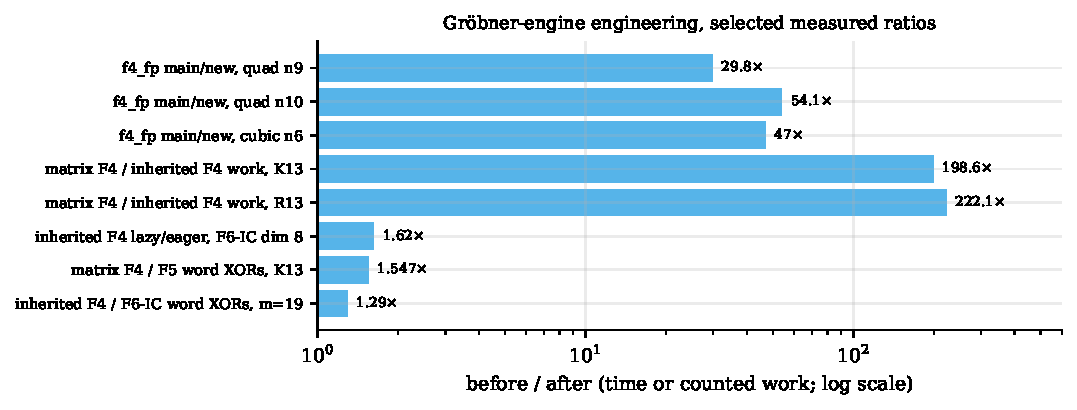
\includegraphics[width=\linewidth]{figures/fig-engine.pdf}
\caption[]{Selected engine ratios (before/after or baseline/candidate):
\texttt{f4\_fp} successive versions (single-threaded wall, L0); matrix
versus inherited F4 (counted matrix work); lazy versus eager inherited
rewrite (median wall); F4 versus F5 and inherited F4 versus F6-IC (word
XORs, stage only). Sources in \art{figures/data.json}.}
\label{fig:engine}
\end{figure}

\paragraph{What did not work.} Degree-2 early-abort probes after a
2025--26 proposal: word-XOR ratios $1.00083$--$1.00378$ (no change) and
$0.99714$--$0.99928$ (worse). Gate-first geometry: $1.57$--$1.78\times$
fewer word XORs but lane-batched F4 roots cost $2.6$--$4.0\times$ a
sequential control. Convolution splitting of the summation polynomial:
$1.21$--$2.07\times$ \emph{more} word operations despite lower degree;
Frobenius auxiliary variables: $57$--$701\times$ more
(\art{research/lit2026_w\{4,5,8\}_*_20261011/}). Symmetry-breaking clauses
in SAT did not help (\art{RESEARCH_KOBLITZ_INDEX_CALCULUS.md}). A
registered law for the $m=3$ refutation degree resolved all 68 units but
ended with the verdict ``neither'': one variant met its generic degree
window on 32/32 draws, the other fell below it on 8, and the heaviest
degree-10 Macaulay solves were $2.4\cdot10^5\times2.0\cdot10^5$ matrices at
42--51 minutes each (\art{research/ic_semiregular_law_20261005/}).
